\chapter{Introdução}

A sedimentação consiste principalmente na separação de uma suspensão de um sólido disperso num líquido por diferença de densidade, com o auxílio do campo gravitacional. Os equipamentos industriais usados para esta finalidade são conhecidos genericamente como sedimentadores, sendo que, dependendo da finalidade, estes podem ser chamados de clarificadores, quando se deseja um líquido límpido, ou espessadores, quando o sólido retido é o produto de interesse \citep{pecanha, unicamp}.
Geometricamente, o sedimentador é um tanque cilíndrico com base cônica, na qual entra uma corrente de alimentação (A) e saem duas correntes, o passante (P) e o retido (R). Operacionalmente, este equipamento pode ser utilizado em processos contínuos ou em batelada \citep{pecanha, unicamp}. Dentre as mais comuns aplicações estão: a remoção de areia e sólidos grosseiros em tratamento de água, na indústria de mineração para separação da lama de minérios, na tratamento de efluentes na indústria têxtil e de papel e celulose, entre outros.
Nesta prática, partiu-se de uma suspensão de carbonato de cálcio a qual foi homogeneizada por agitação e colocada numa proveta, com a qual se observou a sedimentação gradual dos sólidos. A partir do que foi observado, tem-se como objetivo projetar um sedimentador em escala industrial.


\chapter{Descrição Teórica do Sistema}


Para se projetar um sedimentador industrial é preciso determinar a área e a altura deste, com base no valor de concentração da alimentação e a concentração desejada na saída do sedimentador. Para isso, é necessário realizar testes de proveta para determinar alguns parâmetros em escala de laboratório.

Durante os testes de proveta, utiliza-se uma suspensão com as mesmas condições de temperatura e pH que são encontradas nos processo industrial. O teste de proveta permite obter a curva de posição da interface em função do tempo. A partir dessa curva, são obtidos parâmetros \emph{cinéticos} que permitem estimar a área e altura do sedimentador industrial.


\section{Etapas de Sedimentação e o teste da proveta}

Durante o processo de sedimentação, quatro zonas são formadas e nos testes de proveta realizados em escala de bancada, elas não são muito bem definidas. A fim de entender melhor como ocorre o mecanismo da sedimentação e como ela ocorre ao passar do tempo, pode-se analisar a Figura \ref{etapasprov}.


\begin{figure}[H]
	\begin{center}
		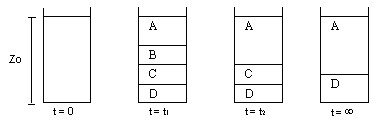
\includegraphics[scale=.8, trim={0 0 0 0}]{figuras/ladeq/sedi/proveta}
		%\vspace{-20pt}
		\caption{Mecanismo de sedimentação.}
		\label{etapasprov}
	\end{center}
\end{figure}


No início da decantação (t = 0), a suspensão encontra-se a uma altura $ Z_{0} $ e sua concentração é uniforme. Pouco tempo depois ($t = t_{1} $) é possível distinguir quatro zonas distintas. São elas:


\begin{itemize}
\item A - Líquido Clarificado: esta camada pode ficar turva durante certo tempo devido à presença de partículas mais finas que permanecem em suspensão;
\item B - Região de Concentração constante ou concentração inicial: tem-se a sedimentação livre, isto é, desconsideram-se os efeitos de concentração, como se as partículas sedimentassem de forma isolada;
\item C - Região de Concentração Variável: nesta região a concentração da suspensão aumenta gradativamente, variando da concentração inicial até a concentração da suspensão espessada, e já se observa o efeito da concentração;
\item D - Região de Lama (compactação): à medida que ocorre a sedimentação a espessura desta região aumenta. 
\end{itemize}

À medida que a sedimentação ocorre, as regiões A e D tornam-se mais importantes e as regiões B e C tendem a desaparecer. 
A velocidade de sedimentação aumenta na região de clarificado (aceleração) e, a partir deste ponto, permanece constante até o final da região B. A velocidade tende a diminuir (desaceleração) em seguida até alcançar o ponto crítico de sedimentação, momento em que a região B desaparece \citep{macabe}.

Esse comportamento pode ser observado na Figura \ref{sedimentaP}.


\begin{figure}[H]
	\begin{center}
		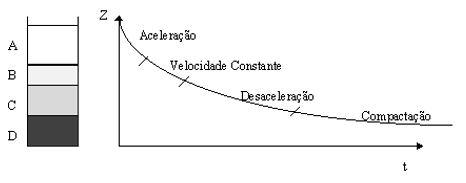
\includegraphics[scale=.8,trim={0 0 0 0}]{figuras/ladeq/sedi/graphProv}
		%\vspace{-20pt}
		\caption{Processo de Sedimentação.}
		\label{sedimentaP}
	\end{center}
\end{figure}

O ponto crítico pode ser determinado, pois enquanto a região B, de concentração igual à inicial, ainda existe, a velocidade de sedimentação é constante e, assim, a variação da altura da interface com o tempo é linear. Porém, ao B desaparecer, a velocidade de sedimentação começa a variar, devido ao fato da concentração também ser variável. Conforme a concentração aumentar, a velocidade de sedimentação diminui, como ilustrado na Figura \ref{linearReg}.


\begin{figure}[H]
	\begin{center}
		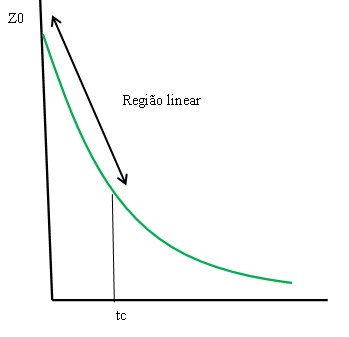
\includegraphics[scale=.5,trim={0 0 0 0}]{figuras/ladeq/sedi/graphProv2}
		%\vspace{-20pt}
		\caption{Determinação gráfica do tempo crítico (tC).}
		\label{linearReg}
	\end{center}
\end{figure}

\section{Balanço de Massa}

Um sedimentador, com suas respectivas correntes e concentrações, é representado no esquema da Figura \ref{esquema}.

\begin{figure}[H]
	\begin{center}
		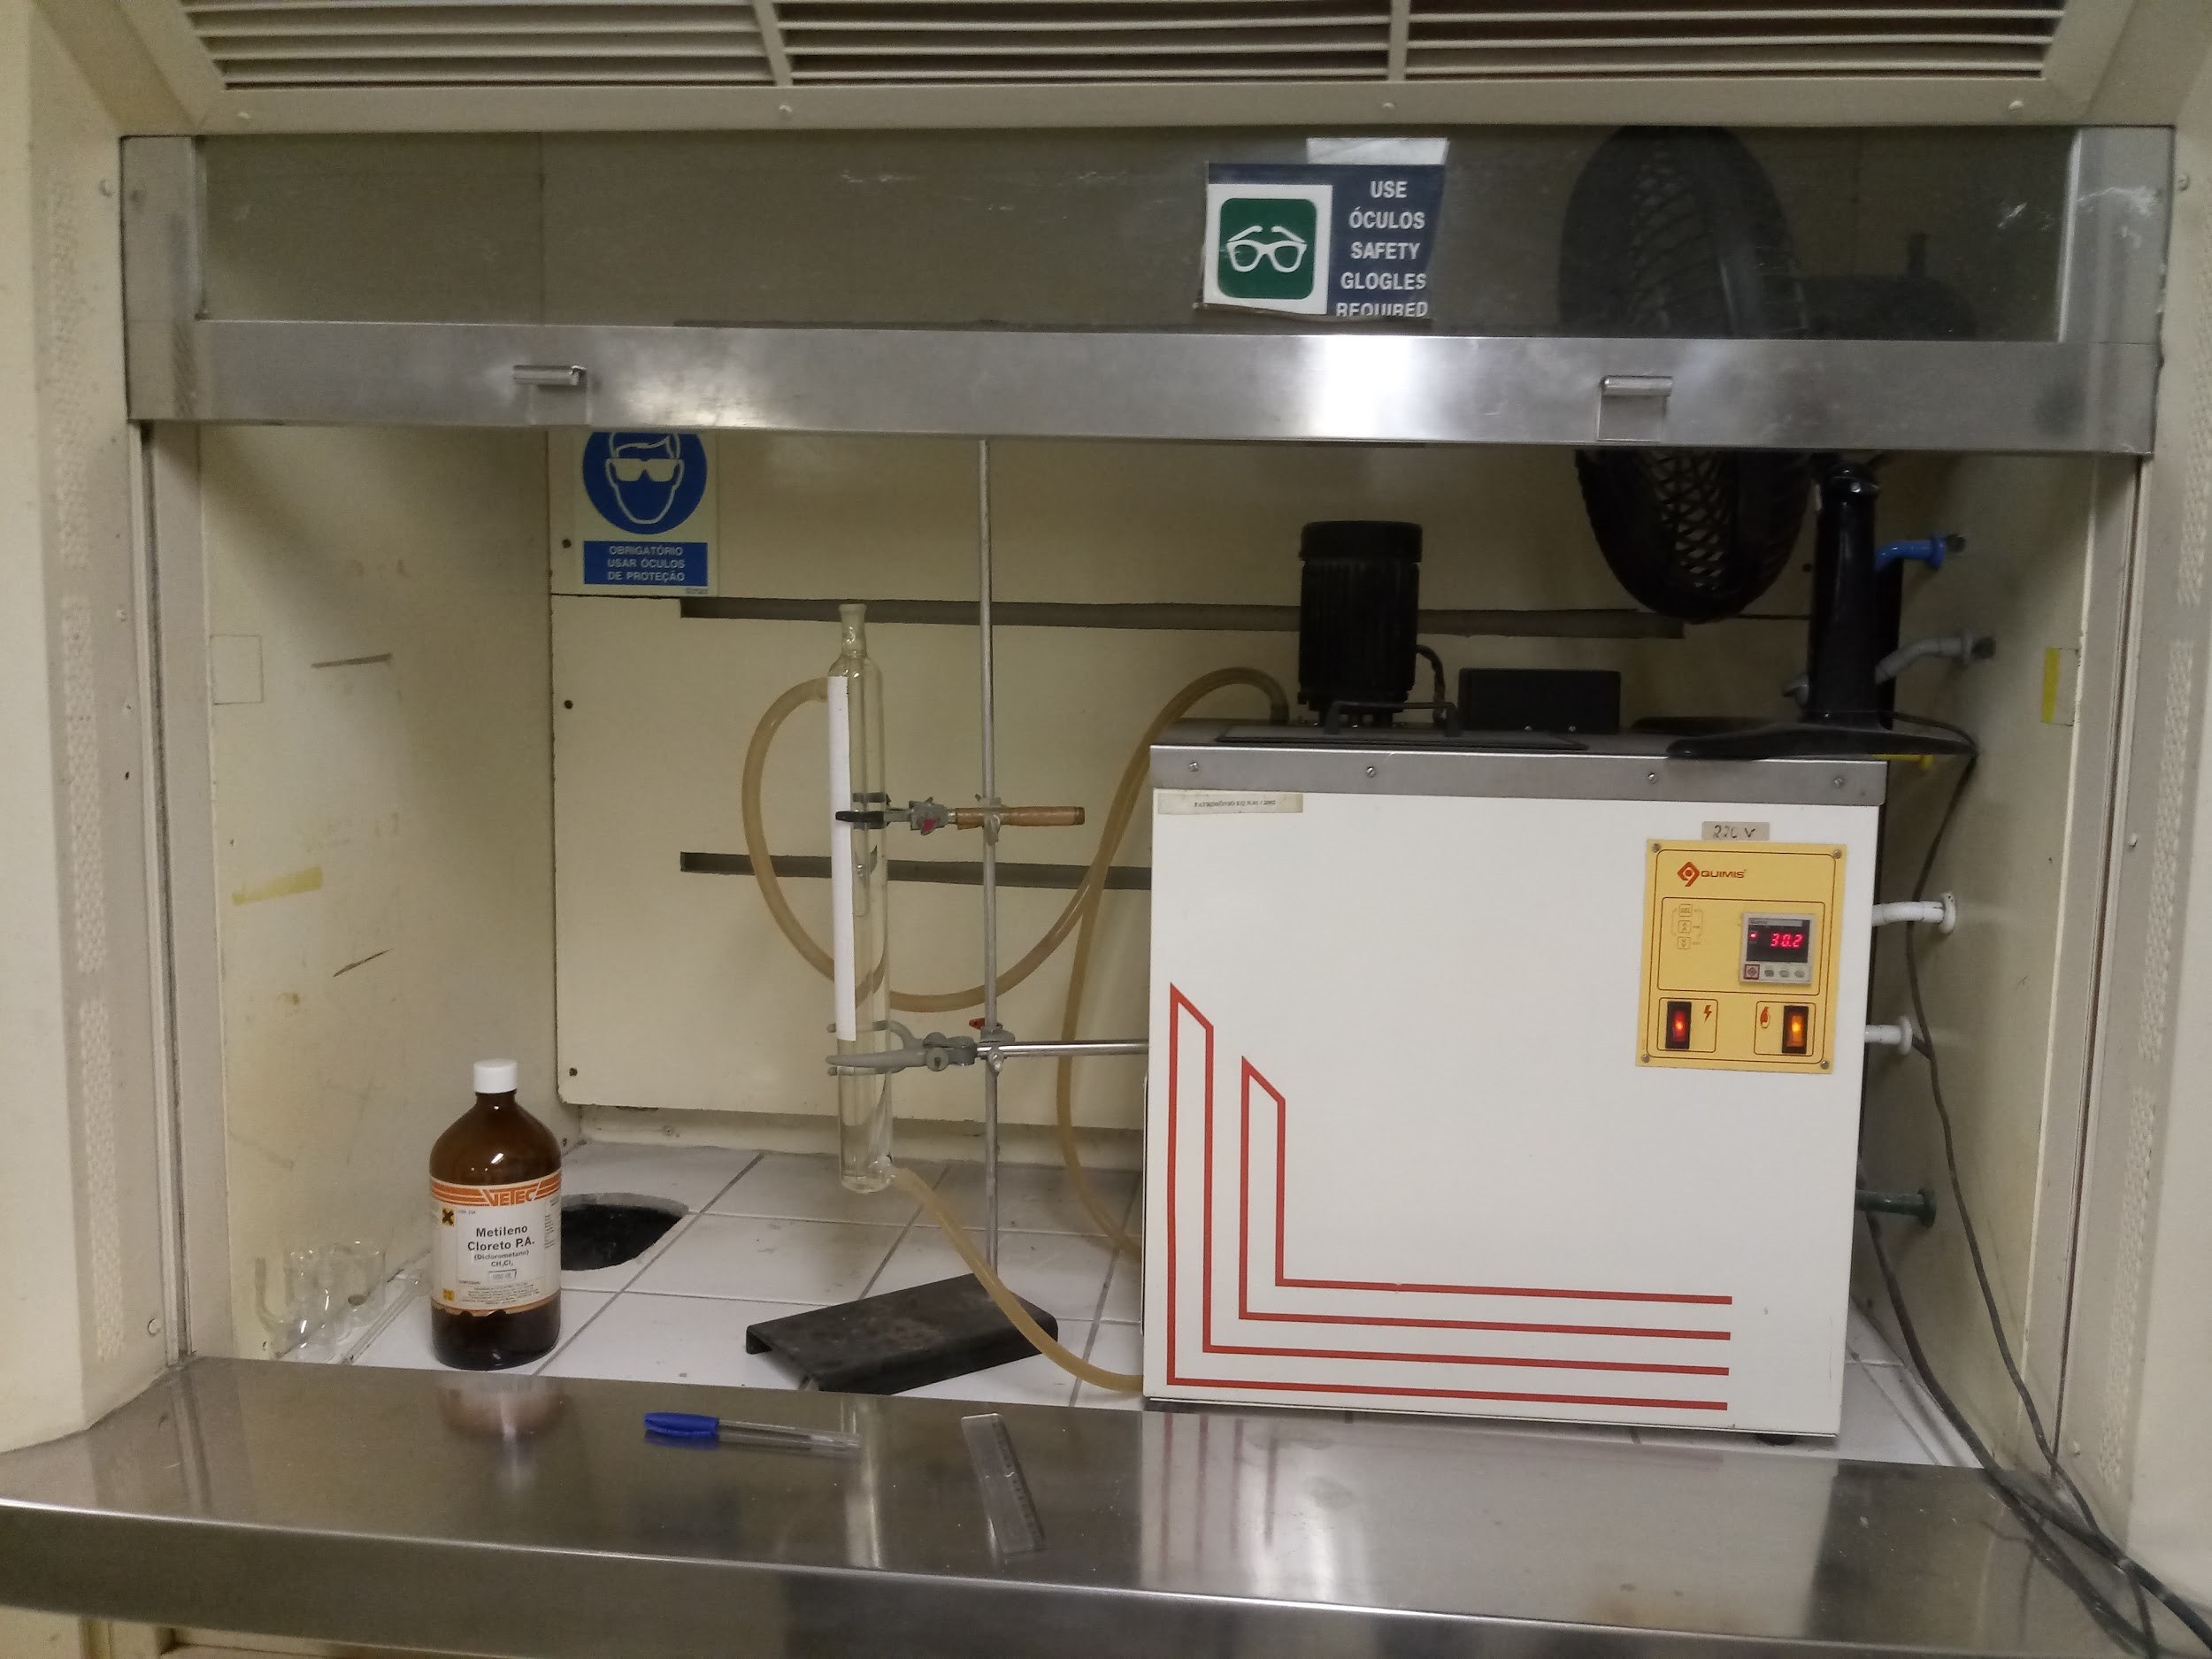
\includegraphics[scale=.5,trim={0 0 0 0}]{figuras/ladeq/sedi/aparato}
		%\vspace{-20pt}
		\caption{Esquema de um sedimentador e suas variáveis.}
		\label{esquema}
	\end{center}
\end{figure}

Em que:

\begin{itemize}
\item Q – Vazão da alimentação
\item $ C_{v} $ – Concentração volumétrica de sólidos na alimentação
\item $ Q_{o} $ – Vazão volumétrica do overflow (líquido clarificado)
\item $ C_{vo} $ – Concentração volumétrica de sólidos no overflow
\item $ Q_{u} $ – Vazão volumétrica do underflow (sólidos concentrados, “lama”)
\item $ C_{vu }$ – Concentração volumétrica de sólidos no underflow
\item $ Q_{a} $ – Vazão volumétrica de líquido límpido no nível L em sentido ascendente
\item $ Q_{L} $ – Vazão volumétrica no nível L em sentido descendente
\item $ C_{vL} $ – Concentração de sólidos no nível L em sentido descendente
\end{itemize}



Para se iniciar o balanço de massa, considera-se que a concentração de sólidos na corrente de líquido clarificado é igual à zero. Logo, a vazão ascendente consiste apenas de líquido clarificado $ (C_{V0} = 0) $. Portanto, temos o seguinte balanço de massa para os sólidos:

\begin{equation}\label{key}
\rho s \times Q \times C v=\rho s \times Q u \times C v u=\rho s \times Q_{L} \times C v L
\end{equation}


Sendo $\rho_{S}$ a densidade das partículas sólidas. Portanto:

\begin{equation}\label{key}
\mathrm{Qu}=\mathrm{Q} \times \frac{\mathrm{Cv}}{\mathrm{Cvu}}
\end{equation}

Já para o líquido, temos o seguinte balanço de massa, no nível L:

\begin{equation}\label{key}
\rho \times \mathrm{Q}_{L} \times(1-\mathrm{CvL})=\rho \times \mathrm{Qa}+\rho \times \mathrm{Qu} \times(1-\mathrm{Cvu})
\end{equation}

Sendo $\rho$ a densidade do líquido. 
Assim,

\begin{equation}\label{key}
\mathrm{Qu}=\frac{\mathrm{Q}_{L} \times \mathrm{CvL}}{\mathrm{Cvu}}
\end{equation}

\begin{equation}\label{key}
Q_{L} \times(1-C v L)=Q a+\frac{Q_{L} \times C_{V L}}{C v u} \times(1-C v u)
\end{equation}

\begin{equation}\label{key}
\mathrm{Qa}=\mathrm{Q}_{L}-\mathrm{Q}_{L} \times \mathrm{CvL}-\frac{\mathrm{Q}_{L} \times \mathrm{CvL}}{\mathrm{Cvu}}+\mathrm{Q}_{L} \times \mathrm{CvL}
\end{equation}

\begin{equation}\label{key}
\mathrm{Q}_{L} \times \mathrm{CvL}=\mathrm{Q} \times \mathrm{Cv}
\end{equation}

\begin{equation}\label{key}
\mathrm{Qa}=\mathrm{Q}_{\mathrm{L}}-\frac{\mathrm{Q}_{L} \times \mathrm{CVL}}{\mathrm{Cvu}}=\mathrm{Q}_{L} \times \operatorname{CvL} \times\left(\frac{1}{\mathrm{CVL}}-\frac{1}{\mathrm{Cvu}}\right)
\end{equation}

\begin{equation}\label{key}
\mathrm{Qa}=\mathrm{Q} \times \mathrm{Cv} \times\left(\frac{1}{\mathrm{CvL}}-\frac{1}{\mathrm{Cvu}}\right)
\end{equation}

\begin{equation}\label{key}
\frac{\mathrm{Qa}}{\mathrm{A}}=\frac{\mathrm{Q} \times \mathrm{Cv}}{\mathrm{A}} \times\left(\frac{1}{\mathrm{CvL}}-\frac{1}{\mathrm{Cvu}}\right)
\end{equation}

A hipótese do método de Coe e Clevenger se baseia na sedimentação das partículas. Este método foi o primeiro a ser desenvolvido e é a fundamentação dos demais.Ele parte da ideia de que todas as partículas alimentadas devem seguir para zona de espessado. Caso isto não ocorra, acarretará no acúmulo de partículas, devido ao arraste, numa dada região chamada de zona limite.

Para tanto, tomando como base que $ C_{V0} = 0 $, a velocidade de ascensão do líquido deve ser menor que a velocidade de sedimentação das partículas, evitando, assim, que elas sejam arrastadas no sentido ascendente. Portanto, deve-se ter:



\begin{equation}\label{key}
\frac{\mathrm{Qa}}{\mathrm{A}} \leq \mathrm{v}
\end{equation}

Onde: $ \frac{Qa}{A} = $ velocidade de ascensão do fluido e v = velocidade de sedimentação das partículas.

No limite, tem-se:

\begin{equation}\label{key}
\frac{\mathrm{Qa}}{\mathrm{A}}=\mathrm{v}
\end{equation}

Assim:

\begin{equation}\label{key}
\frac{\mathrm{Q} \times \mathrm{Cv}}{\mathrm{A}} \times\left(\frac{1}{\mathrm{CvL}}-\frac{1}{\mathrm{Cvu}}\right)=\mathrm{v}
\end{equation}

Chegamos, então, à fórmula da área mínima:

\begin{equation}\label{key}
\mathrm{A}=\frac{\mathrm{Q} \times \mathrm{C} \mathrm{v}}{\mathrm{v}} \times\left(\frac{\mathrm{1}}{\mathrm{C} \mathrm{v} \mathrm{L}}-\frac{\mathrm{1}}{\mathrm{C} \mathrm{v} \mathrm{u}}\right)
\end{equation}


\section{Método de Kynch}

Kynch desenvolveu um método de dimensionamento de sedimentadores que necessita de apenas um ensaio experimental, diferentemente do método de Cloe e Clevenger, que exige inúmeros experimentos. 

O ensaio é iniciado com uma concentração uniforme $ C_{0} $. Supondo que, numa determinada seção do decantador, onde a concentração possui um valor C, a capacidade do equipamento passa por um mínimo e chega até um máximo quando o sistema está em operação, é nesse momento que uma zona característica começará a se formar nessa seção \citep{foust}. 

Se a seção transversal S for insuficiente,ocorrerá acúmulo de sólidos e a zona limite será deslocada para mais perto da saída de clarificado. Mas se a área for suficiente, em regime permanente, os sólidos que entram no sistema também saem.


O procedimento proposto por Kynch requer apenas um ensaio de decantação que forneça a curva de decantação (Z em função de t), através do qual se traçam tangentes em diversos pontos da curva e determinam-se os valores de t, Z e $ Z_{i} $. Com esses valores (t, Z e $ Z_{i} $), utiliza-se a expressão do método de Coe e Clevenger para obter as áreas da seção transversal.

O valor máximo de área obtida corresponderá à área mínima que o decantador poderá ter.

O método gráfico pode ser verificado na Figura \ref{met}.

\begin{figure}[H]
	\begin{center}
		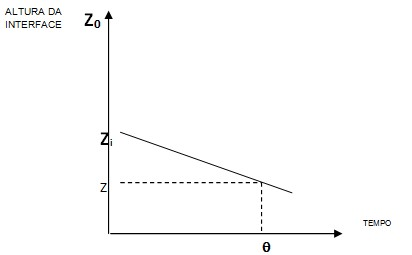
\includegraphics[scale=.5,trim={0 0 0 0}]{figuras/ladeq/sedi/graphKynch}
		%\vspace{-20pt}
		\caption{Exemplo de resultado do método de Kynch.}
		\label{met}
	\end{center}
\end{figure}


A reta tangente pode ser obtida após o cálculo de cada derivada, para cada altura da interface de sedimentação z, correspondente a um tempo de sedimentação t, utilizando as fórmulas a seguir:

\begin{equation}\label{key}
z=\frac{\mathrm{d} z}{\mathrm{dt}} \mathrm{t}+\mathrm{zi} \quad \quad \mathrm{zi}=z-\frac{\mathrm{d} z}{\mathrm{dt}} \mathrm{t}
\end{equation}

Assim, a concentração de sólidos em um nível L qualquer $ C_{vL} $ pode ser calculada, a partir dos valores de $ z_{i} $ correspondentes a cada altura da interface z, através da seguinte relação:

\begin{equation}\label{key}
\mathrm{C_{vL}}=\mathrm{C_{v}} \times \frac{\mathrm{z} _{0}}{\mathrm{z_{i}}}
\end{equation}

Finalmente, calcula-se a área mínima do sedimentador pela equação obtida pelo balanço de massa realizado acima:

\begin{equation}\label{key}
\operatorname{A_{min}}=\frac{\mathrm{Q} \times \mathrm{C_{v}}}{\mathrm{v}} \times\left(\frac{1}{\mathrm{C_{vL}}}-\frac{1}{\mathrm{C_{vU}}}\right)
\end{equation}

No final do experimento, tem-se um conjunto de áreas mínimas calculadas, que podem ser organizadas em uma tabela como a representada abaixo:

	

\begin{table}[H]
	\centering
	\begin{tabular}{|l|l|l|l|l|l|}
		\hline
		\textbf{t} & \textbf{z} & $ \mathbf{\left( \dfrac{d z}{dt} \right)} $ & \textbf{zi} & $ \mathbf{C_{vL}} $ & \textbf{A} \\ \hline
		t1 & z1 & $ \left ( \dfrac{d z}{dt}\right )_{1} $ & zi1 & CvL1 & A1 \\ \hline
		t2 & z2 & $ \left ( \dfrac{d z}{dt} \right )_{2} $ & zi2 & CvL2 & A2 \\ \hline
		... & ... & ... & ... & ... & ... \\ \hline
		tn & zn & $ \left ( \dfrac{d z}{dt}\right )_{n} $ & zin & CvLn & An \\ \hline
	\end{tabular}
	\caption{Organização dos dados no método de Kynch.}
	\label{kynch}
\end{table}


Dentre todas as áreas mínimas calculadas pelo método de Kynch, a de maior valor deve ser utilizada como base de cálculo da área de projeto.


\section{Método de Biscaia Jr.}

Esse método é relativamente mais simples do que o método de Kynch. No método de Biscaia Jr., assume-se que a curva da altura da interface em função do tempo pode ser representada por uma função composta, sendo a primeira parte da curva linear e a segunda exponencial. 

$ Z_{\text{mín}} $ tem seu valor determinado a partir da seguinte relação:

\begin{equation}\label{key}
Z_{\min }=z_{0} * \frac{\mathrm{CvO}}{\mathrm{Cvu}}
\end{equation}

E com o valor de $ z_{\text{mín }}$, através do gráfico da Figura \ref{tabqua1}, obtém-se o valor de $ t_{\text{mín}} $.

\begin{figure}[H]
	\begin{center}
		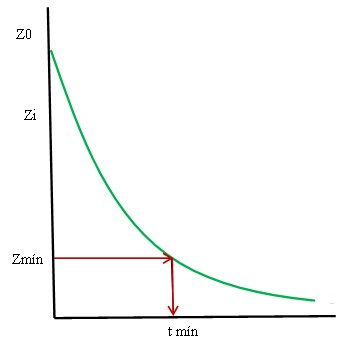
\includegraphics[scale=.5,trim={0 0 0 0}]{figuras/ladeq/sedi/graphBiscaia}
		%\vspace{-20pt}
		\caption{Representação gráfica do método de Biscaia Jr.}
		\label{tabqua1}
	\end{center}
\end{figure}


Com o valor detmín obtido, pode-se então determinar $ A_{\text{mín}} $:

\begin{equation}\label{key}
\operatorname{A_{\text{mín}}}=Q \times \frac{t_{\text{mín}}}{z_{0}}
\end{equation}


\section{Fatores de Correção}

A área determinada por ambos os métodos é a área mínima que o sedimentador deve ter para que se tenha a sedimentação desejada. Porém, é necessário o ajuste de alguns parâmetros para reproduzir as condições operacionais de um sedimentador industrial mais fielmente.


\begin{equation}\label{key}
A_{proj}=\operatorname{A_{\text{mín}}} \times \mathrm{f}_{1} \times \mathrm{f}_{2}
\end{equation}

O fator $ f_{1} $considera efeitos de pH, temperatura, diâmetro dos flocos e concentração das partículas. Esse fator é especialmente importante em locais onde há grande variação de temperatura.

\begin{equation}\label{key}
1,10 \leq f_{1} \leq 1,25
\end{equation}


Já o fator $ f_{2} $ é função do diâmetro das partículas e considera a turbulência causada pela alimentação da suspensão no sedimentador. Como a velocidade nos tubos de alimentação é muito maior que a velocidade dentro do sedimentador, há geração de uma zona de turbulência na região de alimentação, dificultando a sedimentação. O fator de segurança visa amortecer o efeito da zona de turbulência através do aumento do diâmetro.

\begin{equation}\label{key}
1,10 \mathrm{m}<\mathrm{D}_{\mathrm{min}}<1,25 \mathrm{m} \quad 1,2 \leq \mathrm{f}_{2} \leq 1,5
\end{equation}

\begin{equation}\label{key}
D_{\min } \leq 5 \mathrm{m} \quad \mathrm{f}_{2}=1,5
\end{equation}

\begin{equation}\label{key}
\mathrm{D}_{\mathrm{min}} \geq 30 \mathrm{m} \quad \mathrm{f}_{2}=1,2
\end{equation}


\chapter{Objetivo}


O experimento tem como objetivo determinar o dimensionamento de um sedimentador a partir dos dados coletados em um teste de proveta para a suspensão de $ CaCO_{3} $, utilizando os métodos de Kynch e Biscaia Jr. e fazer comparações com os valores obtidos.

O sedimentador industrial deverá operar com uma suspensão de carbonato de cálcio, de aproximadamente 3,9\% em peso de $ CaCO_{3} $, para obtenção de uma lama de concentração de sólidos 2 vezes superior à da alimentação.
\\


\chapter{Materiais e Métodos}

\section{Materiais}

\begin{itemize}
\item Suspensão de carbonato de cálcio;
\item 1 Proveta graduada de 2L;
\item 3 Vidros de relógio;
\item Pipeta;
\item Bastão de Vidro;
\item Balança analítica digital;
\item Cronômetro;
\item Tira de papel milimetrado;
\item Estufa.
\end{itemize}

\section{Métodos}

Realizou-se o teste de proveta usando 2 L da suspensão de carbonato de cálcio. Para determinar a concentração real da suspensão, antes do início do teste, colocou-se 3 amostras em vidros de relógios secos previamente pesados. Após a adição da suspensão, os vidros foram novamente pesados. As amostras foram à estufa por, aproximadamente, $ 100^{\circ} $C até peso constante e então novamente os vidros foram pesados.


O teste de proveta iniciou assim que os 2L de solução estavam bem homogeneizados na proveta, com o auxílio do bastão de vidro, iniciando o cronômetro. A sedimentação iniciou e foi possível observar a formação de 2 fases, uma mais opaca com alto teor de sólidos e uma clarificada. A interface foi monitorada e o tempo anotado a cada decréscimo da mesma em 0,5 cm de altura. Com os pontos, foi possível plotar o gráfico $ Z \times t $.




\chapter{Resultados e Discussão}

\section{Propriedades físico-químicas}

\begin{itemize}
\item Densidade da água$ (\rho): 1 \ \dfrac{g}{cm^{3}} $
\item Densidade do carbonato de cálcio $ (\rho _{S}): 2,711 \ \dfrac{g}{cm^{3}} $ (a $ 25^{\circ} $C)
\item Viscosidade da água $ (\mu): 0,01 \ \dfrac{g \cdot cm}{s}$ 
\end{itemize}




\section{Determinação da concentração e densidade de $ \mathbf{CaCO_{3}} $ na suspensão}


Para determinação das concentrações mássica e volumétrica, utilizaram-se os dados da Tabela \ref{param}.


\begin{table}[H]
	\centering
	\begin{tabular}{|c|c|c|c|}
		\hline
		\textbf{Numeração} & \textbf{\begin{tabular}[c]{@{}c@{}}M1: Vidro de\\ relógio vazio\\ (g)\end{tabular}} & \textbf{\begin{tabular}[c]{@{}c@{}}M2: Vidro de relógio\\ com suspensão inicial\\ (g)\end{tabular}} & \textbf{\begin{tabular}[c]{@{}c@{}}M3: Vidro de relógio\\ com suspensão seca \\ (g)\end{tabular}} \\ \hline
		\textbf{S1} & 36,0549 & 39,6448 & 39,1954 \\ \hline
		\textbf{S2} & 44,723 & 48,1705 & 44,8572 \\ \hline
		\textbf{S3} & 36,0498 & 39,6998 & 36,1928 \\ \hline
	\end{tabular}
	\caption{Tabela com as massas em cada etapa do procedimento.}
	\label{param}
\end{table}



A partir dos resultados experimentais, os cálculos realizados foram: $ H_{2}O $ e $ CaCO_{3} $ foram determinados do seguinte modo:






\begin{itemize}
\item Massa de $ H_{2}O: M_{2} -M_{3} $
\item Massa de $ CaCO_{3}: M_{3}-M_{1} $
\end{itemize}

\subsection{Cálculos}

Determinar a concentração mássica significa efetuar a seguinte razão:
\begin{equation}\label{key}
\mathrm{C}_{m}=\frac{\text { massa de sólido }\left(\mathrm{CaCO}_{3}\right)}{\text { massa de suspensão }}=\frac{\text { massa de sólido }\left(\mathrm{CaCO}_{3}\right)}{\text { massa de água }+\text { massa de } \mathrm{CaCO}_{3}}
\end{equation}


%Determinar a concentração volumétrica significa efetuar:
%
%\begin{equation}\label{key}
%C_{V}=\frac{ V_{\text{sólido}} \left(\mathrm{CaCO}_{3}\right)}{V_{\text{suspensão}}}
%\end{equation}
%
%
%\begin{equation}\label{key}
%\mathrm{V}_{ \text {sólido}}=\frac{\text { massa sólidos }\left(\mathrm{CaCO}_{3}\right)}{\rho_{S}}
%\end{equation}
%
%
%\begin{equation}\label{key}
%V_{\text{suspensão}} = V_{\text{água}}+V_{\text{sólidos}}
%\end{equation}
%
%
%\begin{equation}\label{key}
%V_{\text{suspensão}} = \dfrac{ \text{massa água} }{\rho}+\dfrac{\text { massa sólidos (CaCO }_{3} )}{\rho_{s}}
%\end{equation}
%
%
%\begin{equation}\label{key}
%\mathrm{C}_{V}=\frac{\frac{\text { massa sólidos }}{\rho_{S}}}{\frac{\text { massa água }}{\rho}+\frac{\text { massa sólidos }}{\rho_{S}}}
%\end{equation}
%
%Determinar a densidade da suspensão significa efetuar:
%
%\begin{equation}\label{key}
%\rho_{\text { suspensäo }}=\frac{\text { massa suspensão }}{\mathrm{V} \text { suspensão }}
%\end{equation}
%
%\begin{equation}\label{key}
%\rho_{\text { suspensão }}=\frac{\text { massa suspensão }}{\text { volume } \mathrm{CaCO}_{3}+\text { volume } \mathrm{H_{2} O}}
%\end{equation}
%
%
%\begin{equation}\label{key}
%\rho_{\text { suspensão }}=\frac{\text { massa suspensão }}{\frac{\text { massa }CaCO_{3}}{\rho_{S}}+\frac{\text { massa } \mathrm{H_{2} O}}{\rho}}
%\end{equation}


\begin{table}[H]
	\centering
	\begin{tabular}{|c|c|c|c|}
		\hline
		\textbf{Numeração} & \textbf{\begin{tabular}[c]{@{}c@{}}Massa Úmida\\ g\end{tabular}} & \textbf{\begin{tabular}[c]{@{}c@{}}Massa Seca\\ g\end{tabular}} & \textbf{\% Sólidos} \\ \hline
		S1 & 3,5899 & 0,1405 & 0,0391 \\ \hline
		S2 & 3,4475 & 0,1342 & 0,0389 \\ \hline
		S3 & 3,6500 & 0,143 & 0,0392 \\ \hline
	\end{tabular}
	\caption{Concentração de sólidos nas alíquotas coletadas.}
	\label{alim}
\end{table}


Para os demais cálculos foi utilizada a média das concentrações obtidas através da alíquotas coletadas da suspensão de alimentação do teste de proveta. O valor médio calculado foi igual a 3,91 \% p de sólidos.

\section{Teste de Proveta}

\subsection{Altura inicial da proveta}

Sabendo-se que a $ \text{Área} = \dfrac{\pi D^{2}}{4} $ e $ Volume = \text{Área} \cdot Z_{0} $, temos:

\begin{table}[H]
	\centering
	\begin{tabular}{|c|c|}
		\hline
		\textbf{\begin{tabular}[c]{@{}c@{}}Diâmetro da proveta\\ (cm)\end{tabular}} & 8,1 \\ \hline
		\textbf{\begin{tabular}[c]{@{}c@{}}Área da seção transversal \\ da proveta (cm²)\end{tabular}} & 51,53 \\ \hline
		\textbf{\begin{tabular}[c]{@{}c@{}}Volume inicial \\ (cm³ = mL)\end{tabular}} & 2000 \\ \hline
		\textbf{\begin{tabular}[c]{@{}c@{}}Altura inicial \\ de líquido (cm)\end{tabular}} & 38,81 \\ \hline
	\end{tabular}
	\caption{Dados do sistema montado para o teste de proveta.}
	\label{dadosprov}
\end{table}


\subsection{Curva de sedimentação (altura da proveta x tempo)}

Uma vez iniciada a sedimentação, o grupo anotou o tempo para a suspensão sedimentar a cada 0,5 cm, obtendo a seguinte curva:


\begin{figure}[H]
	\begin{center}
		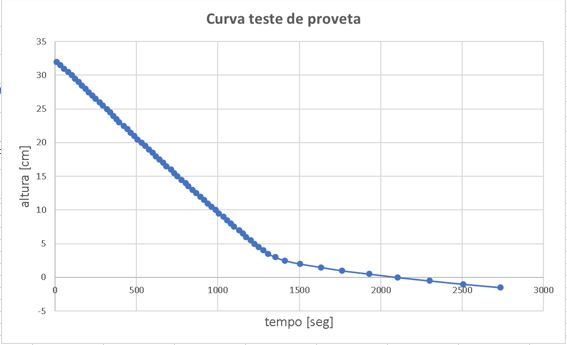
\includegraphics[scale=.9,trim={0 0 0 0}]{figuras/ladeq/sedi/alturatempo}
		%\vspace{-20pt}
		\caption{Curva obtida para os dados de sedimentação.}
		\label{tabqua1}
	\end{center}
\end{figure}


Diante da curva apresentada, efetuaram-se dois ajustes, um linear, inicialmente, e um exponencial. Considerou-se adequado, uma vez que os coeficientes de correlação estão próximos a 1. Com as equações ajustadas, utilizaram-se os métodos para determinação da área do sedimentador. 

\begin{figure}[H]
	\begin{center}
		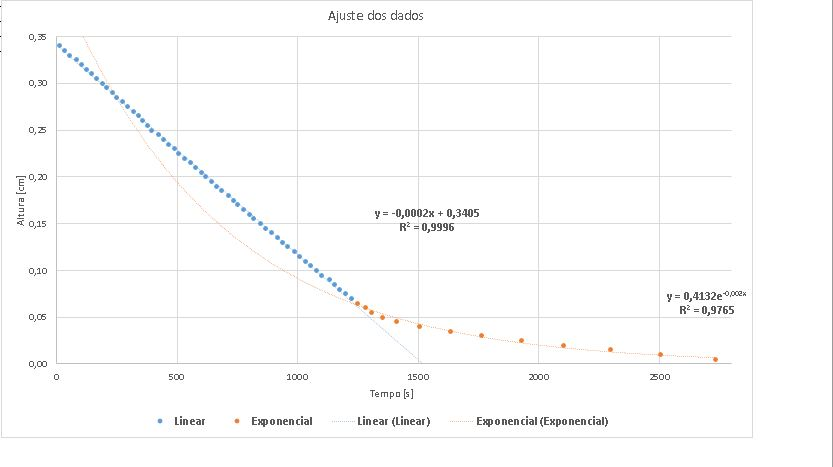
\includegraphics[scale=.7,trim={0 0 0 0}]{figuras/ladeq/sedi/ajuste}
		%\vspace{-20pt}
		\caption{Curva obtida para os dados de sedimentação.}
		\label{tabqua1}
	\end{center}
\end{figure}


\subsection{Calculo das vazões para dimensionamento do sedimentador}

Com base nos seguintes dados para uma operação industrial, projetou-se um sedimentador industrial com base no teste de proveta.


\begin{itemize}
\item Vazão da unidade industrial: 36 ton/h;
\item Concentração desejada de carbonato de calcio na lama: 5\% em peso;
\item Concentração do carbonato da cálcio na alimentação: 2,5 \%.
\item Concentração do carbonato da cálcio na alimentação: 3,9 \%.
\end{itemize}

Vazões volumétrica, vazão mássica e concentração de sólidos da suspensão utilizada na alimentação do teste de proveta podem ser observadas na Tabela \ref{tabalim}, para o retido na Tabela \ref{tabretido} e o passante na Tabela \ref{passan}

\begin{table}[H]
	\centering
	\begin{tabular}{|c|c|c|c|c|c|}
		\hline
		\textbf{} & \textbf{\begin{tabular}[c]{@{}c@{}}Dens\\ (kg/m³)\end{tabular}} & \textbf{\begin{tabular}[c]{@{}c@{}}CA\\ (\%)\end{tabular}} & \textbf{\begin{tabular}[c]{@{}c@{}}QA\\ (kg/h)\end{tabular}} & \textbf{\begin{tabular}[c]{@{}c@{}}QA\\ m³/h\end{tabular}} & \textbf{\begin{tabular}[c]{@{}c@{}}CA\\ (kg/m³)\end{tabular}} \\ \hline
		CaCO3 & 2730 & 3,9\% & 1406,9091 & 0,52 & 40,07 \\ \hline
		H2O & 1000 & 96,1\% & 34593,091 & 34,59 & 985,32 \\ \hline
		TOTAL & & 100,0\% & 36000 & 35,11 & 1.025,39 \\ \hline
	\end{tabular}
	\caption{Vazões e concentração na alimentação do sedimentador que será projetado.}
	\label{tabalim}
\end{table}


\begin{table}[H]
	\centering
	\begin{tabular}{|c|c|c|c|c|c|}
		\hline
		\textbf{} & \textbf{\begin{tabular}[c]{@{}c@{}}Dens\\ (kg/m³)\end{tabular}} & \textbf{CR (\%)} & \textbf{\begin{tabular}[c]{@{}c@{}}QR \\ (kg/h)\end{tabular}} & \textbf{\begin{tabular}[c]{@{}c@{}}QR\\ m3/h\end{tabular}} & \textbf{\begin{tabular}[c]{@{}c@{}}CR\\ (kg/m³)\end{tabular}} \\ \hline
		CaCO3 & 2730 & 15,6\% & 1406,9091 & 0,52 & 173,51 \\ \hline
		H2O & 1000 & 84,4\% & 7593,0909 & 7,59 & 936,44 \\ \hline
		TOTAL & & 100,0\% & 9000 & 8,11 & 1.109,95 \\ \hline
	\end{tabular}
	\caption{Vazões e concentração no retido do sedimentador que será projetado.}
	\label{tabretido}
\end{table}


\begin{table}[H]
	\centering
	\begin{tabular}{|c|c|c|c|c|c|}
		\hline
		\textbf{} & \textbf{\begin{tabular}[c]{@{}c@{}}Dens\\ (kg/m³)\end{tabular}} & \textbf{CP} & \textbf{\begin{tabular}[c]{@{}c@{}}QP\\ kg/h\end{tabular}} & \textbf{\begin{tabular}[c]{@{}c@{}}QP\\ m³/h\end{tabular}} & \textbf{\begin{tabular}[c]{@{}c@{}}CP\\  kg/m3\end{tabular}} \\ \hline
		CaCO3 & 2730 & 0,00\% & 0,00 & 0,00 & 0,00 \\ \hline
		H2O & 1000 & 100,00\% & 27.000,00 & 27,00 & 1.000,00 \\ \hline
		TOTAL & & 100,00\% & 27.000,00 & 27,00 & 1.000,00 \\ \hline
	\end{tabular}
	\caption{Vazões e concentração no passante do sedimentador que será projetado.}
	\label{passan}
\end{table}



\subsection{Método de Kynch}

Segundo o método de Kynch, a área mínima do sedimentador pode ser calculada pela equação abaixo:

\begin{equation}\label{key}
\frac{\mathrm{Q}_{\mathrm{L}} \mathrm{C}_{\mathrm{L}}}{\mathrm{S}}=\frac{\mathrm{v}_{\mathrm{L}}}{\left(\frac{1}{\mathrm{C}_{\mathrm{L}}}-\frac{1}{\mathrm{C}_{\mathrm{R}}}\right) \frac{<\rho^{\prime}>}{\rho_{\mathrm{P}}}}
\end{equation}


%\begin{equation}\label{key}
%\mathrm{A} \min =\frac{\mathrm{Q} * \mathrm{C}_{V}}{\mathrm{v}} *\left(\frac{1}{\mathrm{C}_{V L}}-\frac{1}{\mathrm{C}_{V U}}\right)
%\end{equation}
%
%Onde:
%
%\begin{itemize}
%	\item $ \mathrm{Q}=\frac{Q_{\text { mássica }}}{ P_{\text{suspensão }}} $;
%	\item $ C_{V} $ Concentração volumétrica de alimentação;
%	\item $ v=\frac{-d z}{d t} $
%	\item $ \mathrm{C}_{V L}=\mathrm{C}_{V} * \frac{\mathrm{z}_{0}}{\mathrm{z}_{I}} $
%	\item $ \mathrm{z}_{I}=\mathrm{z}-\frac{\mathrm{d} z}{\mathrm{dt}} * \mathrm{t} $
%
%\end{itemize}


Resumo das informações sobre vazão e concentração obtidos pelo teste de proveta.


\begin{table}[H]
	\centering
	\begin{tabular}{|c|c|c|c|}
		\hline
		\textbf{Corrente} & \textbf{\begin{tabular}[c]{@{}c@{}}Q\\ $ m^{3}/h $\end{tabular}} & \textbf{\begin{tabular}[c]{@{}c@{}}C\\ $ kg/m^{3} $\end{tabular}} & \textbf{\begin{tabular}[c]{@{}c@{}}Dens\\ $ kg/m^{3} $\end{tabular}} \\ \hline
		\textbf{A} & 35,11 & 40,07 & 1.025,39 \\ \hline
		\textbf{R} & 8,11 & 173,51 & 1.109,95 \\ \hline
		\textbf{P} & 27,00 & 0 & 1.000,00 \\ \hline
	\end{tabular}
	\caption{Resumo das vazões e concentrações do sedimentador que será projetado.}
	\label{resumo}
\end{table}

Utilizandos os dados da Tabela \ref{resumo}, calculou-se a densidade média através da Equação \ref{eita}.

\begin{equation}\label{eita}
<\rho>=\frac{\rho_{\mathrm{A}} \mathrm{C}_{\mathrm{R}}-\rho_{\mathrm{R}} \mathrm{C}_{\mathrm{A}}}{\mathrm{C}_{\mathrm{R}}-\mathrm{C}_{\mathrm{A}}}
\end{equation}


\begin{table}[H]
	\centering
	\begin{tabular}{|c|c|c|}
		\hline
		\textbf{C0} & 40,07 & \textbf{kg/m³} \\ \hline
		\textbf{z0} & 0,34 & \textbf{m} \\ \hline
		\textbf{\textless{}dens\textgreater{}} & 1000 & \textbf{kg/m³} \\ \hline
	\end{tabular}
	\caption{Densidade média.}
	\label{rhomedio}
\end{table}



\subsubsection{Tabela com os valores calculados para área}

\begin{equation}\label{key}
\frac{\mathrm{Q}_{\mathrm{L}} \mathrm{C}_{\mathrm{L}}}{\mathrm{S}}=\frac{\mathrm{v}_{\mathrm{L}}}{\left(\frac{1}{\mathrm{C}_{\mathrm{L}}}-\frac{1}{\mathrm{C}_{\mathrm{R}}}\right) \frac{<\rho^{\prime}>}{\rho_{\mathrm{P}}}}
\end{equation}


\begin{table}[H]
	\centering
	\begin{tabular}{|c|c|c|c|c|c|c|c|}
		\hline
		\textbf{\begin{tabular}[c]{@{}c@{}}tL\\ s\end{tabular}} & \textbf{Geral} & \textbf{Derivada} & \textbf{\begin{tabular}[c]{@{}c@{}}vL\\ m/s\end{tabular}} & \textbf{\begin{tabular}[c]{@{}c@{}}ziL\\ m\end{tabular}} & \textbf{\begin{tabular}[c]{@{}c@{}}CL\\ kg/m³\end{tabular}} & \textbf{\begin{tabular}[c]{@{}c@{}}QL\\ CL/S\end{tabular}} & \textbf{\begin{tabular}[c]{@{}c@{}}A\\ m²\end{tabular}} \\ \hline
		10 & 0,340 & -4,45E-04 & 4,45E-04 & 0,344 & 3,96E+01 & 0,02281 & 17,13 \\ \hline
		31 & 0,335 & -4,36E-04 & 4,36E-04 & 0,349 & 3,91E+01 & 0,02200 & 17,76 \\ \hline
		54 & 0,330 & -4,26E-04 & 4,26E-04 & 0,353 & 3,86E+01 & 0,02115 & 18,48 \\ \hline
		80 & 0,325 & -4,15E-04 & 4,15E-04 & 0,358 & 3,80E+01 & 0,02022 & 19,33 \\ \hline
		102 & 0,320 & -4,06E-04 & 4,06E-04 & 0,361 & 3,77E+01 & 0,01956 & 19,98 \\ \hline
		123 & 0,315 & -3,98E-04 & 3,98E-04 & 0,364 & 3,74E+01 & 0,01898 & 20,59 \\ \hline
		145 & 0,310 & -3,89E-04 & 3,89E-04 & 0,366 & 3,72E+01 & 0,01841 & 21,23 \\ \hline
		163 & 0,305 & -3,82E-04 & 3,82E-04 & 0,367 & 3,71E+01 & 0,01803 & 21,68 \\ \hline
		188 & 0,300 & -3,73E-04 & 3,73E-04 & 0,370 & 3,68E+01 & 0,01742 & 22,44 \\ \hline
		206 & 0,295 & -3,66E-04 & 3,66E-04 & 0,370 & 3,68E+01 & 0,01708 & 22,87 \\ \hline
		230 & 0,290 & -3,57E-04 & 3,57E-04 & 0,372 & 3,66E+01 & 0,01658 & 23,57 \\ \hline
		249 & 0,285 & -3,51E-04 & 3,51E-04 & 0,372 & 3,66E+01 & 0,01626 & 24,04 \\ \hline
		273 & 0,280 & -3,42E-04 & 3,42E-04 & 0,373 & 3,65E+01 & 0,01581 & 24,72 \\ \hline
		293 & 0,275 & -3,35E-04 & 3,35E-04 & 0,373 & 3,65E+01 & 0,01551 & 25,20 \\ \hline
		319 & 0,270 & -3,27E-04 & 3,27E-04 & 0,374 & 3,64E+01 & 0,01506 & 25,95 \\ \hline
		338 & 0,265 & -3,21E-04 & 3,21E-04 & 0,373 & 3,65E+01 & 0,01482 & 26,37 \\ \hline
		357 & 0,260 & -3,15E-04 & 3,15E-04 & 0,372 & 3,66E+01 & 0,01459 & 26,78 \\ \hline
		376 & 0,255 & -3,09E-04 & 3,09E-04 & 0,371 & 3,67E+01 & 0,01438 & 27,18 \\ \hline
		\end{tabular}
	\caption{}
\label{tabelakynch}
\end{table}
		
		\begin{table}[H]
			\centering
			\begin{tabular}{|c|c|c|c|c|c|c|c|}
		394 & 0,250 & -3,03E-04 & 3,03E-04 & 0,369 & 3,69E+01 & 0,01420 & 27,52 \\ \hline
		421 & 0,245 & -2,95E-04 & 2,95E-04 & 0,369 & 3,69E+01 & 0,01383 & 28,25 \\ \hline
		444 & 0,240 & -2,88E-04 & 2,88E-04 & 0,368 & 3,70E+01 & 0,01357 & 28,79 \\ \hline
		465 & 0,235 & -2,82E-04 & 2,82E-04 & 0,366 & 3,72E+01 & 0,01337 & 29,23 \\ \hline
		487 & 0,230 & -2,76E-04 & 2,76E-04 & 0,365 & 3,74E+01 & 0,01316 & 29,69 \\ \hline
		506 & 0,225 & -2,71E-04 & 2,71E-04 & 0,362 & 3,76E+01 & 0,01302 & 30,01 \\ \hline
		530 & 0,220 & -2,65E-04 & 2,65E-04 & 0,360 & 3,78E+01 & 0,01280 & 30,53 \\ \hline
		554 & 0,215 & -2,58E-04 & 2,58E-04 & 0,358 & 3,80E+01 & 0,01259 & 31,04 \\ \hline
		576 & 0,210 & -2,53E-04 & 2,53E-04 & 0,356 & 3,83E+01 & 0,01243 & 31,44 \\ \hline
		599 & 0,205 & -2,47E-04 & 2,47E-04 & 0,353 & 3,86E+01 & 0,01226 & 31,87 \\ \hline
		619 & 0,200 & -2,42E-04 & 2,42E-04 & 0,350 & 3,89E+01 & 0,01216 & 32,14 \\ \hline
		642 & 0,195 & -2,37E-04 & 2,37E-04 & 0,347 & 3,93E+01 & 0,01201 & 32,53 \\ \hline
		664 & 0,190 & -2,32E-04 & 2,32E-04 & 0,344 & 3,96E+01 & 0,01189 & 32,86 \\ \hline
		682 & 0,185 & -2,27E-04 & 2,27E-04 & 0,340 & 4,01E+01 & 0,01184 & 32,99 \\ \hline
		712 & 0,180 & -2,21E-04 & 2,21E-04 & 0,337 & 4,04E+01 & 0,01163 & 33,61 \\ \hline
		732 & 0,175 & -2,16E-04 & 2,16E-04 & 0,333 & 4,09E+01 & 0,01157 & 33,79 \\ \hline
		752 & 0,170 & -2,12E-04 & 2,12E-04 & 0,329 & 4,14E+01 & 0,01151 & 33,95 \\ \hline
		775 & 0,165 & -2,07E-04 & 2,07E-04 & 0,326 & 4,19E+01 & 0,01143 & 34,20 \\ \hline
		801 & 0,160 & -2,02E-04 & 2,02E-04 & 0,322 & 4,24E+01 & 0,01131 & 34,55 \\ \hline
		818 & 0,155 & -1,98E-04 & 1,98E-04 & 0,317 & 4,29E+01 & 0,01132 & 34,52 \\ \hline
		845 & 0,150 & -1,93E-04 & 1,93E-04 & 0,313 & 4,35E+01 & 0,01121 & 34,85 \\ \hline
		868 & 0,145 & -1,89E-04 & 1,89E-04 & 0,309 & 4,41E+01 & 0,01117 & 35,00 \\ \hline
		892 & 0,140 & -1,84E-04 & 1,84E-04 & 0,304 & 4,48E+01 & 0,01112 & 35,15 \\ \hline
		915 & 0,135 & -1,80E-04 & 1,80E-04 & 0,300 & 4,54E+01 & 0,01109 & 35,24 \\ \hline
		938 & 0,130 & -1,76E-04 & 1,76E-04 & 0,295 & 4,62E+01 & 0,01107 & 35,29 \\ \hline
						\end{tabular}
	\caption{}
\label{tabelakynch}
\end{table}

\begin{table}[H]
\centering
\begin{tabular}{|c|c|c|c|c|c|c|c|}
		959 & 0,125 & -1,72E-04 & 1,72E-04 & 0,290 & 4,69E+01 & 0,01109 & 35,24 \\ \hline
		985 & 0,120 & -1,68E-04 & 1,68E-04 & 0,285 & 4,77E+01 & 0,01106 & 35,34 \\ \hline
		1006 & 0,115 & -1,64E-04 & 1,64E-04 & 0,280 & 4,86E+01 & 0,01110 & 35,22 \\ \hline
		1033 & 0,110 & -1,60E-04 & 1,60E-04 & 0,275 & 4,95E+01 & 0,01108 & 35,27 \\ \hline
		1055 & 0,105 & -1,57E-04 & 1,57E-04 & 0,270 & 5,04E+01 & 0,01113 & 35,11 \\ \hline
		1079 & 0,100 & -1,53E-04 & 1,53E-04 & 0,265 & 5,14E+01 & 0,01117 & 34,98 \\ \hline
		1100 & 0,095 & -1,50E-04 & 1,50E-04 & 0,260 & 5,25E+01 & 0,01126 & 34,71 \\ \hline
		1130 & 0,090 & -1,45E-04 & 1,45E-04 & 0,254 & 5,36E+01 & 0,01127 & 34,68 \\ \hline
		1152 & 0,085 & -1,42E-04 & 1,42E-04 & 0,249 & 5,48E+01 & 0,01138 & 34,35 \\ \hline
		1174 & 0,080 & -1,39E-04 & 1,39E-04 & 0,243 & 5,60E+01 & 0,01150 & 33,98 \\ \hline
		1200 & 0,075 & -1,35E-04 & 1,35E-04 & 0,238 & 5,74E+01 & 0,01161 & 33,67 \\ \hline
		1225 & 0,070 & -1,32E-04 & 1,32E-04 & 0,232 & 5,88E+01 & 0,01174 & 33,29 \\ \hline
		1250 & 0,065 & -1,29E-04 & 1,29E-04 & 0,226 & 6,03E+01 & 0,01190 & 32,84 \\ \hline
		1280 & 0,060 & -1,25E-04 & 1,25E-04 & 0,220 & 6,19E+01 & 0,01204 & 32,47 \\ \hline
		1308 & 0,055 & -1,22E-04 & 1,22E-04 & 0,214 & 6,37E+01 & 0,01222 & 31,97 \\ \hline
		1352 & 0,050 & -1,16E-04 & 1,16E-04 & 0,207 & 6,57E+01 & 0,01231 & 31,75 \\ \hline
		1410 & 0,045 & -1,10E-04 & 1,10E-04 & 0,200 & 6,82E+01 & 0,01233 & 31,69 \\ \hline
		1504 & 0,040 & -9,99E-05 & 9,99E-05 & 0,190 & 7,16E+01 & 0,01218 & 32,08 \\ \hline
		1633 & 0,035 & -8,78E-05 & 8,78E-05 & 0,178 & 7,64E+01 & 0,01198 & 32,63 \\ \hline
		1762 & 0,030 & -7,72E-05 & 7,72E-05 & 0,166 & 8,21E+01 & 0,01202 & 32,51 \\ \hline
		1931 & 0,025 & -6,52E-05 & 6,52E-05 & 0,151 & 9,03E+01 & 0,01227 & 31,84 \\ \hline
		2105 & 0,020 & -5,48E-05 & 5,48E-05 & 0,135 & 1,01E+02 & 0,01314 & 29,74 \\ \hline
		2299 & 0,015 & -4,51E-05 & 4,51E-05 & 0,119 & 1,15E+02 & 0,01528 & 25,57 \\ \hline
		2508 & 0,010 & -3,66E-05 & 3,66E-05 & 0,102 & 1,34E+02 & 0,02140 & 18,26 \\ \hline
		2736 & 0,005 & -2,92E-05 & 2,92E-05 & 0,085 & 1,61E+02 & 0,06366 & 6,14 \\ \hline
	\end{tabular}
	\caption{}
	\label{tabelakynch}
\end{table}


\subsubsection{Fatores de correção}

\begin{table}[H]
	\centering
	\begin{tabular}{|c|c|c|c|c|c|c|}
		\hline
		\textbf{\begin{tabular}[c]{@{}c@{}}mín\\ (\textgreater{}0)\end{tabular}} & \textbf{\begin{tabular}[c]{@{}c@{}}A\\ m²\end{tabular}} & \textbf{\begin{tabular}[c]{@{}c@{}}D\\ m\end{tabular}} & \textbf{\begin{tabular}[c]{@{}c@{}}D\\ ft\end{tabular}} & \textbf{f1} & \textbf{f2} & \textbf{\begin{tabular}[c]{@{}c@{}}A corr.\\ m²\end{tabular}} \\ \hline
		1,11E-02 & 35,34 & 6,71 & 22,01 & 1,18 & 1,30 & 53,98 \\ \hline
	\end{tabular}
	\caption{}
	\label{correo}
\end{table}



\subsection{Método de Biscaia Jr.}

\subsubsection{Determinação de $ \mathbf{Z_{\text{mín}}} $ e $ \mathbf{t_{\text{mín}}} $}


\begin{equation}\label{key}
Z_{\text{mín}} =\mathrm{Z}_{0} * \frac{\mathrm{C}_{A}}{\mathrm{C}_{R}}
\end{equation}

\begin{table}[H]
	\centering
	\begin{tabular}{|c|c|}
		\hline
		\textbf{CA kg/m³} & 40,07 \\ \hline
		\textbf{CR kg/m³} & 173,51 \\ \hline
		\textbf{z0 (m)} & 0,34 \\ \hline
		\textbf{z mín (m)} & 0,08 \\ \hline
	\end{tabular}
	\caption{}
	\label{zmin}
\end{table}

De posse do valor de $ Z_{\text{mín}} $, podemos calcular o valor de $ t_{\text{mín}} $ através da equação obtida pelo ajuste linear.

\begin{table}[H]
	\centering
	\begin{tabular}{|c|c|}
		\hline
		\textbf{a} & 0,3405 \\ \hline
		\textbf{b} & -0,0002 \\ \hline
		\textbf{z mín (m)} & 0,08 \\ \hline
		\textbf{t mín (s)} & 1.309,88 \\ \hline
	\end{tabular}
	\caption{}
	\label{tmin}
\end{table}

\subsubsection{Determinação de $ A_{\text{mín}} $}

\begin{equation}\label{key}
A_{m i n}=Q * \frac{t_{m \hat{m}}}{Z_{0}}
\end{equation}

\begin{table}[H]
	\centering
	\begin{tabular}{|c|c|l|}
		\hline
		\textbf{t mín} & 0,36 & h \\ \hline
		\textbf{z0} & 0,34 & m \\ \hline
		\textbf{QA} & 35,11 & m³/h \\ \hline
		\textbf{S calc} & 37,57 & m² \\ \hline
		\multicolumn{1}{|l|}{\textbf{D calc}} & \multicolumn{1}{l|}{6,92} & m \\ \hline
	\end{tabular}
	\caption{}
	\label{aMIN}
\end{table}







\subsubsection{Fatores de correção}

\begin{table}[H]
	\centering
	\begin{tabular}{|c|c|}
		\hline
		\textbf{D(ft)} & 22,69 \\ \hline
		\textbf{f1} & 1,175 \\ \hline
		\textbf{f2} & 1,3 \\ \hline
		\textbf{A Proj. (m²)} & 57,39 \\ \hline
	\end{tabular}
	\caption{}
	\label{aMIn}
\end{table}



\subsection{Comparação entre os métodos}


\begin{table}[H]
	\centering
	\begin{tabular}{|c|c|c|c|}
		\hline
		\textbf{Método} & \textbf{Kynch} & \textbf{Biscaia Jr.} & \textbf{\begin{tabular}[c]{@{}c@{}}Variação do Kynch em relação ao\\ Biscaia Jr. (\%)\end{tabular}} \\ \hline
		\textbf{Amín (m²)} & 35,34 & 37,57 & 5,947\% \\ \hline
		\textbf{\begin{tabular}[c]{@{}c@{}}Área de\\ projeto (m²)\end{tabular}} & 53,98 & 57,39 & 5,947\% \\ \hline
	\end{tabular}
	\caption{Comparação entre os valores obtidos pelos métodos de Kynch e Biscaia Jr.}
	\label{resumo2}
\end{table}

\chapter{Conclusões}
